\documentclass[varwidth]{standalone}
  \usepackage{amsfonts,amsmath,amssymb}
  \usepackage[slovene]{babel}
  \usepackage[utf8]{inputenc}
  \usepackage[T1]{fontenc}
  
\usepackage{tikz, verbatim, subcaption}
\usepackage{pgfplots}
\usetikzlibrary{arrows.meta, calc, positioning, automata}
\tikzset{point/.style={circle,draw=black,inner sep=0pt,minimum size=2pt}}


\begin{document}



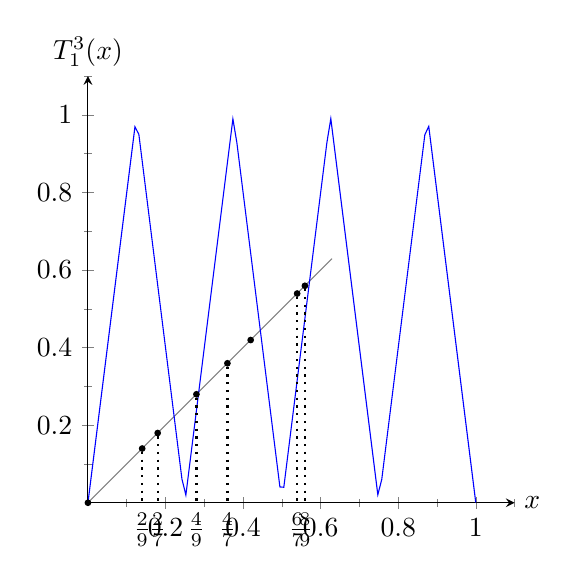
\begin{tikzpicture}
\coordinate (origin) at (0, 0);
\draw[gray] (0, 0) -- (3.1, 3.1);
\begin{axis}[
width=7cm,height=7cm,
minor tick num=1,
axis y line=middle,
axis x line=middle,
xlabel=$x$,ylabel=$T^3_1(x)$,
every axis x label/.style={
    at={(ticklabel* cs:1)},
    anchor=west,
},
every axis y label/.style={
    at={(ticklabel* cs:1)},
    anchor=south,
},
xmin=0,
xmax=1.1,
ymin=0,
ymax=1.1
]
	\addplot[blue,mark=none,
		 domain=-0:1,samples=100] 
		{1-max(2*(1-max(2*(1-max(2*x-1, 1-2*x))-1, 1-2*(1-max(2*x-1, 1-2*x))))-1, 1-2*(1-max(2*(1-max(2*x-1, 1-2*x))-1, 1-2*(1-max(2*x-1, 1-2*x)))))};
\end{axis}
\node[point,fill=black] (a) at (0,0) {};
\node[point,fill=black] (b) at (6.2/9,6.2/9) {};
\node[point,fill=black] (c) at (12.4/9,12.4/9) {};
\node[point,fill=black] (d) at (24.8/9,24.8/9) {};
\node[point,fill=black] (e) at (6.2/7,6.2/7) {};
\node[point,fill=black] (f) at (12.4/7,12.4/7) {};
\node[point,fill=black] (g) at (18.6/7,18.6/7) {};
\node[point,fill=black] (h) at (6.2/3,6.2/3) {};
   	\draw[dotted,thick] (b) -- (b|-origin) node[below] {$\frac{2}{9}$};	
	\draw[dotted,thick] (c) -- (c|-origin) node[below] {$\frac{4}{9}$};
	\draw[dotted,thick] (d) -- (d|-origin) node[below] {$\frac{8}{9}$};
	\draw[dotted,thick] (e) -- (e|-origin) node[below] {$\frac{2}{7}$};
	\draw[dotted,thick] (f) -- (f|-origin) node[below] {$\frac{4}{7}$};
	\draw[dotted,thick] (g) -- (g|-origin) node[below] {$\frac{6}{7}$};
\end{tikzpicture}

\end{document}